\section{The Higgs Mechanism} \label{sec:theory:higgs}

The Higgs Mechanism is the system by which particles attain mass through the
spontaneous breaking of the Higgs potential, thus causing all particles it
interacts with to have mass.

\subsection{Electroweak Symmetry Breaking}

The Higgs field is expressed as a complex doublet, $\boldsymbol{\Phi}$, and thus
has four components as shown in equation \ref{eq:higgs:higgs_field}

\begin{equation} \label{eq:higgs:higgs_field}
\boldsymbol{\Phi}(x) = \left( \begin{matrix} \phi^{+} \\ \phi^{0} \end{matrix}
\right) = \frac{1}{\sqrt{2}} \left( \begin{matrix} \phi_{1}(x) + i\phi_{2}(x) \\
\phi_{3}(x) + i\phi_{4}(x) \end{matrix} \right)
\end{equation}

The four compoenents of this field each represent a degree of freedom which will
be used to give the longitudinal polarizations of the gauge bosons $W^{\pm},Z$
and the mass of the Higgs Boson.  The resulting lagrangian for the higgs
includes a kinetic term (K) as well as the Higgs potential (V) all of which are
invariant under the Electroweak gauge symmetry $SU(2)_L \times U(1)_Y$

\begin{equation}
\mathcal{L}_{\text{Higgs}} =
\underbrace{(D_{\mu}\boldsymbol{\Phi)^{\dagger}}D^{\mu}\boldsymbol{\Phi}}_{\text{K}}
- (\underbrace{\mu^{2}\boldsymbol{\Phi}^{\dagger}\boldsymbol{\Phi} +
  \lambda(\boldsymbol{\Phi}^{\dagger}\boldsymbol{\Phi})^{2}}_{\text{V}})
\end{equation}

Here we constrain $\mu^{2} < 0$ and $\lambda > 0$ such that the potential forms
a stable minima.  The shape of this potential is shown in figure
\ref{fig:higgs_potential} and is often refered to as the "Mexican-hat" or
"Wine-bottle" potential. 

\begin{figure}[!htb]
  \begin{center}
    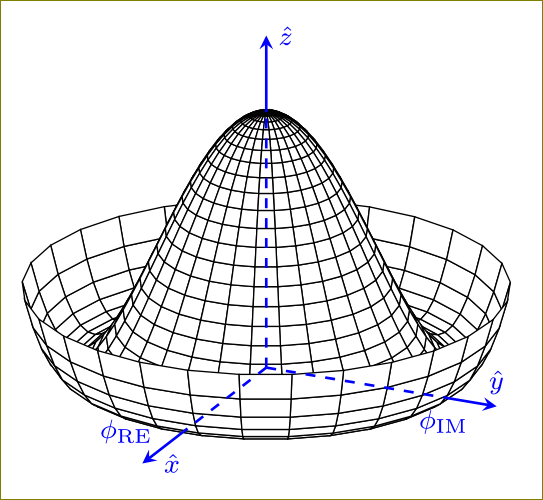
\includegraphics[width=0.6\linewidth]{figures/theory/higgs_potential.png}
    \caption{ A lower dimensionality representation of the shape of the Higgs
Potential.  The central peak represents a $v = 0$ rotationally symmetric
unstable state, while the trough represents the infinite choices of minima that
can be selected upon the spontaneous breaking of symmetry.}
    \label{fig:higgs_potential}
  \end{center}
\end{figure}

Whatever you call it, this potential is significant in
that its minimum is not at $\boldsymbol{\Phi} = 0$ but instead is symmetric
around the origin thus defining an infinite number of states that minimize V.
The value of this minima can be calculated by taking the derivative of V with
respect to $\boldsymbol{\Phi}$ and setting it equal to $0$. This value, also
known as the vacuum expectation value (vev) has been found to be $v \equiv
\sqrt{\mu^{2}/\lambda} = 246$ GeV. In order to reach this ground state energy,
the Higgs field must spontaneously break this symmetry, and thus aquire an
arbitrary single value.  For ease of calculation we orient our coordinate system
such that

\begin{equation}
\left\langle \boldsymbol{\Phi}(x) \right\rangle = \frac{1}{\sqrt{2}} \left(
\begin{matrix} 0 \\ v \end{matrix} \right)
\end{equation} 

Next we parameterize small perturbations around the minimum of the Higgs
potential as 

\begin{equation}
\left\langle \boldsymbol{\Phi}(x) \right\rangle = \frac{1}{\sqrt{2}} \left(
\begin{matrix} 0 \\ v + h(x) \end{matrix} \right) \text{exp} \left(
i\frac{\tau^{i}}{2}\theta^{i}(x) \right)
\end{equation} 

Here the real scalar field $h(x)$ corresponds to radial perturbations of the
minima and while the three $\theta^{i}(x)$ are the Nambu-Goldstone fields with
values determined by your choice of gauge.  Choosing the unitary gauge of
$\theta^{i}(x) = 0$ and expanding the kinetic term around the vev we get

\begin{equation}
\mathcal{L}_{\text{Higgs},K} = \frac{g^{2}v^{2}}{8} \left(
(W_{\mu}^{-})^{\dagger}W^{-\mu} + (W_{\mu}^{+})^{\dagger}W^{+\mu} \right) +
\frac{1}{2} \left( \begin{matrix} W_{\mu}^{3\dagger} & B_{\mu}^{\dagger}
\end{matrix} \right) \boldsymbol{M}^{2} \left( \begin{matrix} W^{3\mu} \\ B^{\mu}
\end{matrix} \right) + \ldots 
\end{equation}

Here the first term is the physical mass term for the $W^{\pm}$ bosons where we
have constructed their charge eigenstates ouf of the $W^{1,2}$ fields like this
$W^{\pm} = \frac{1}{\sqrt{2}}(W^{1} \mp iW^{2}$.  The second term represents the
mixture of the $W^{3}$ and $B$ fields through the mass matrix $\boldsymbol{M}$.
By diagonalizing this matrix and identifying the mass eigenstates we find the
physical fields of the photon ($\gamma$) and the $Z$ boson


\begin{equation}
\boldsymbol{M}_{Diagonalized}^{2} = \left( \begin{matrix} 0 & 0 \\ 0 &
\frac{v^{2}}{4}(g^{2} + g^{'2)}   \end{matrix} \right)
\end{equation}

The upper left diagonal element corresponds to the massless photon
while the lower right diagonal element gives the mass of the massive $Z$ boson.
This leaves us with the following masses for the 4 Electroweak bosons

\begin{equation}
m_{W} = \frac{1}{2}gv \quad , \quad m_Z = \frac{1}{2}v\sqrt{g^{2} + g^{'2}}
\quad , \quad m_\gamma = 0
\end{equation}

The masses of the $W^{\pm}$ and $Z$ gauge bosons can be related through the
Wineberg angle or mixing angle which

\begin{equation}
\theta_W = cos^{-1}\left( \frac{g}{\sqrt{g^{2}+g^{'2}}} \right) \rightarrow m_{Z} =
\frac{m_{W}}{cos{\theta_{W}}}
\end{equation}

Using this definition we can write out the exact mixture of $B$ and $W^{3}$ that
make up the photon and $Z$ boson

\begin{equation}
\gamma = cos(\theta_{W})B + sin(\theta_{W}W^{3})
\end{equation}
\begin{equation}
Z = -sin(\theta_{W})B + cos(\theta_{W}W^{3})
\end{equation}

\subsection{Fermion Mass Terms}

\subsection{The Higgs Boson}


